\chapter{Boolean Algebra}
\label{chap:ch4}
In the previous chapter, we explored various numeral systems — binary, decimal, octal, and hexadecimal — and learned how to perform conversions and binary arithmetic. Binary, with its base-2 structure, is particularly significant in the world of computing because all digital systems operate using binary data. Every number and operation inside a computer is ultimately broken down into a series of 0s and 1s.

As we move from working with binary numbers to understanding \textbf{Boolean algebra}, we take the next step in comprehending how computers perform logical operations using binary values. While numeral systems allowed us to understand how numbers are represented and manipulated, Boolean algebra enables us to understand how decisions and logical processes are carried out within digital systems. In essence, Boolean algebra provides the rules that guide logical decision-making in binary, the same way arithmetic operates in numeral systems.

\section{Introduction to Boolean Algebra}
Boolean algebra is a mathematical framework that deals with binary values — typically represented as 0 and 1 - and shows us what kind of operations that can be carried out on bits. This system, first introduced by \textbf{George Boole} in the mid-19th century, forms the foundation of modern digital logic and is essential in the fields of computer science and electrical engineering.

\begin{figure}[h]
    \centering
    \begin{multicols}{2}  % Split the figure into two columns

        % First image and its caption
        \begin{center}
            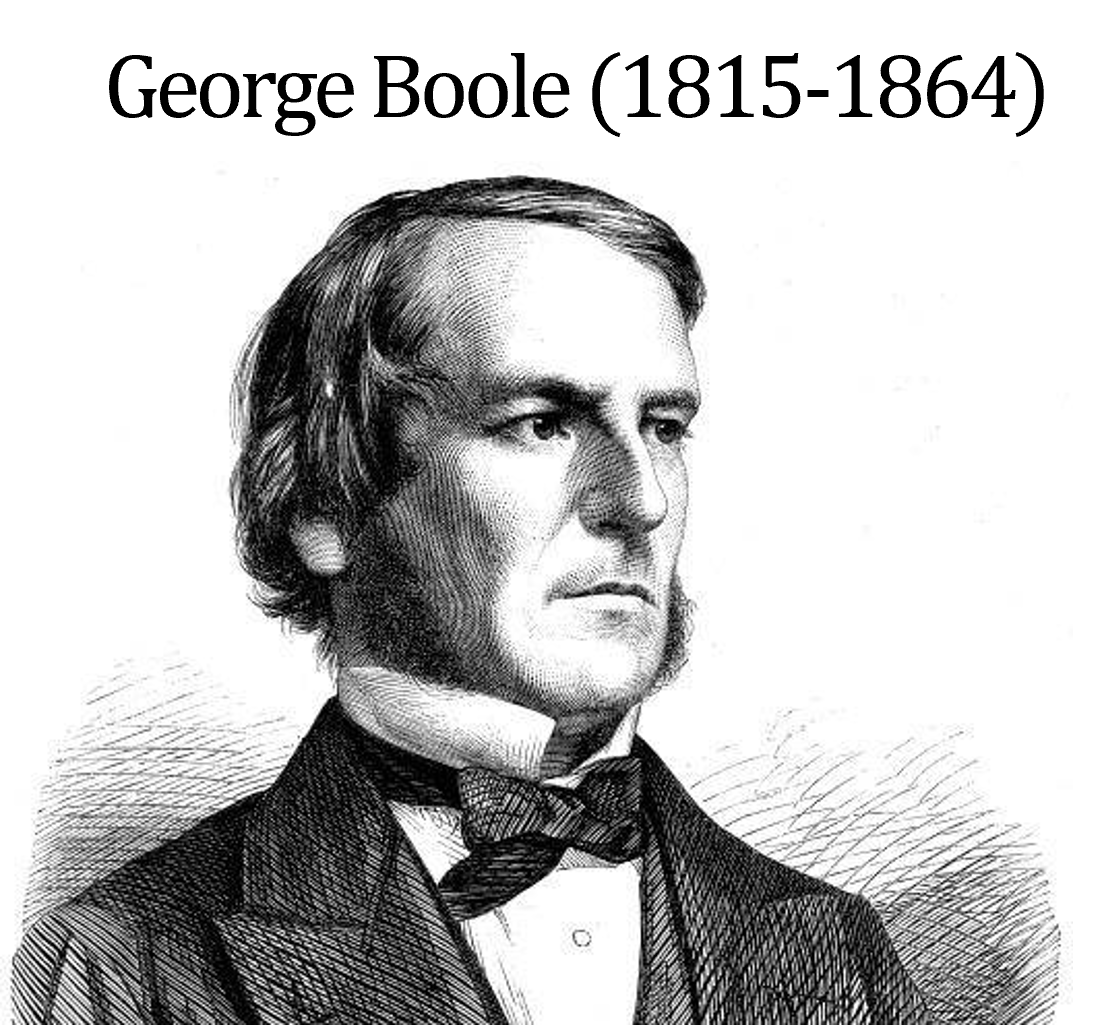
\includegraphics[width=0.6\linewidth]{figure/boole.png}  % Adjust the width as needed
            \caption{Developed the rules of logic.}
        \end{center}

        % Second image and its caption
        \begin{center}
            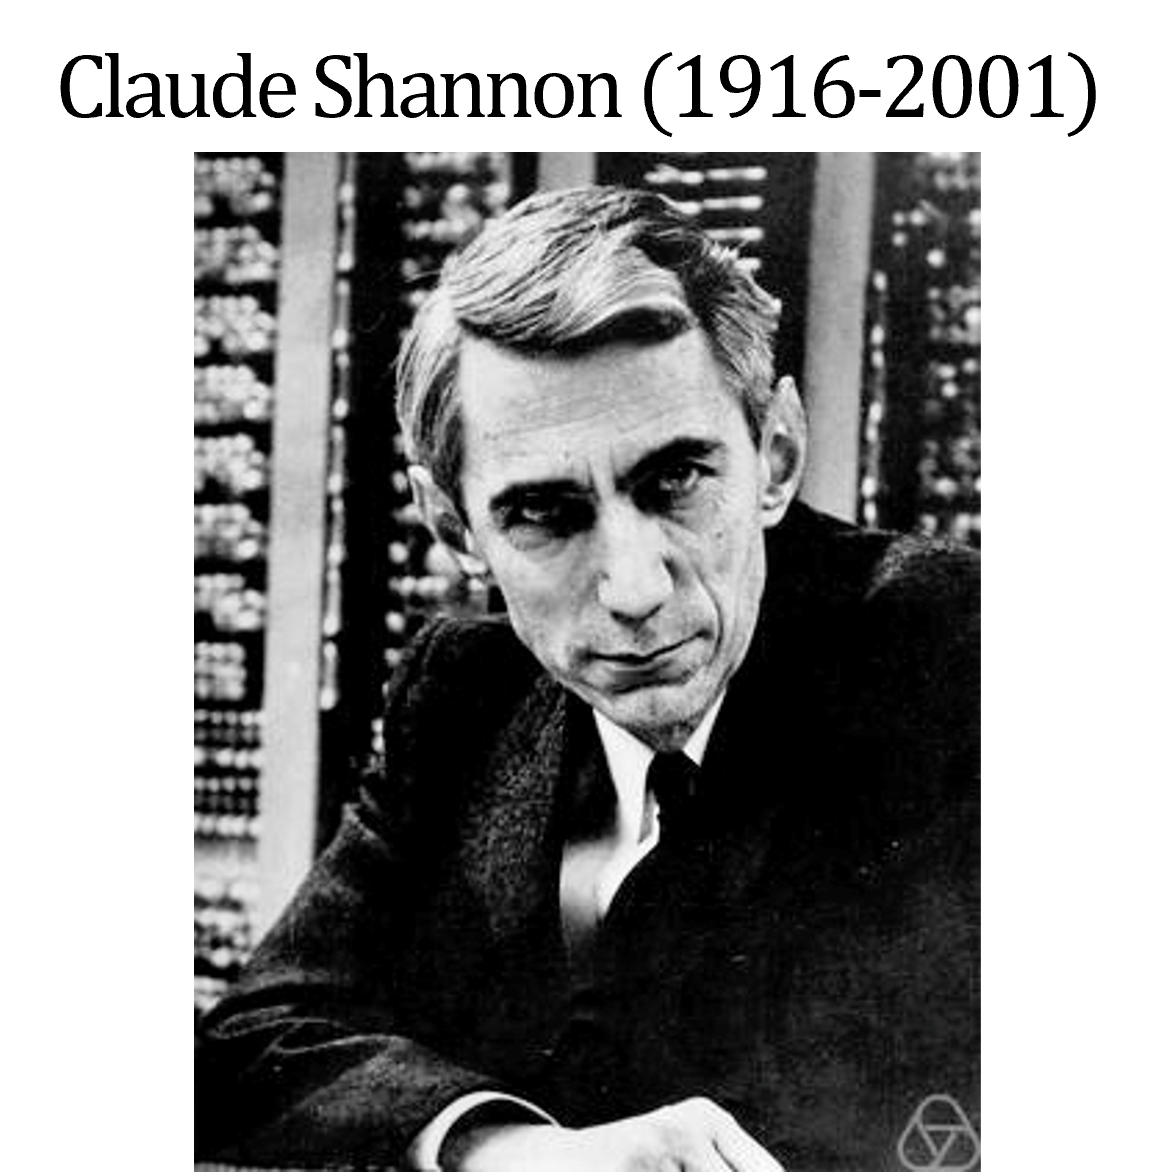
\includegraphics[width=0.6\linewidth]{figure/shannon.png}  % Adjust the width as needed
            \caption{Showed how to use Boolean algebra for designing computer circuits.}
        \end{center}
    \end{multicols}
\end{figure}

Although Boole laid the groundwork, it was not until the 1930s that \textbf{Claude Shannon}, widely regarded as the father of information theory, demonstrated how Boolean algebra could be applied to the design of electronic circuits. In his groundbreaking master's thesis, Shannon showed that Boolean algebra could be used to model and simplify the complex arrangement of switches and relays found in electrical circuits. This revelation bridged the gap between abstract mathematical logic and practical engineering, laying the foundation for the digital circuits used in modern computers. Shannon's master thesis won the 1939 Alfred Noble Prize.

\subsection*{Relevance to Computer Science}
Boolean algebra plays a central role in computer science, especially in the design and functioning of digital systems, such as computers, mobile devices, and embedded systems. At its core, Boolean algebra is used to model and design the behaviour of \textbf{digital circuits}, which are built from electronic components that have two states: on or off, corresponding directly to the binary values 1 and 0.

At the heart of these digital circuits are \textbf{transistors}. A transistor is a tiny electronic device (typically less than 45 nanometres in size) that allows current to flow through it, functioning as a switch. Computers are made up of billions of connected transistors.

\begin{figure}[h]
    \centering
    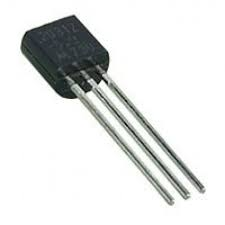
\includegraphics[width = 0.3\textwidth]{figure/transistor.png} % Adjust width here to scale the image
    \caption{A Transistor.}
    \label{fig:transistor}
\end{figure}

These transistors can be wired together in such a way that they store information in binary form — each 0 or 1 represents a single bit of information. Furthermore, they can be used to perform logical operations on these bits.

Every computation or decision made by a computer involves a series of logical operations — such as \texttt{AND}, \texttt{OR}, and \texttt{NOT} — that are described and optimised using Boolean expressions. These logical operations are fundamental to controlling the flow of data and decision-making in software and hardware systems. For example:

\begin{itemize}
    \item In \textbf{processors}, Boolean algebra is used to create \textbf{logic gates} and circuits that handle data processing, arithmetic operations, and decision-making.
    \item In \textbf{software}, conditional statements like \texttt{IF} and \texttt{ELSE} are based on Boolean logic, determining which paths a program will follow.
\end{itemize}

Beyond digital circuits, Boolean algebra also underpins essential concepts in \textbf{logic programming}, \textbf{database querying}, and \textbf{search algorithms}, where conditions must be evaluated as \texttt{TRUE} or \texttt{FALSE}.

At the physical level, the circuits in digital devices operate by processing binary inputs to produce a binary output. Each of these circuits can be modelled using Boolean functions, which are expressions that describe how input values are manipulated to produce an output. For example, a simple \texttt{AND} gate outputs 1 only if both of its inputs are 1, which aligns directly with the Boolean operation \( x \land y \).

Boolean algebra is not only a way of simplifying logical reasoning but also a tool for optimising digital circuit designs. By simplifying Boolean expressions, designers can reduce the number of logic gates required, which leads to more efficient circuits that use less power and occupy less space on a chip.

\section{Basic Operations on Bits}
Boolean operators define the basic rules for manipulating binary values (0 and 1). The three primary operations in Boolean algebra are:

\begin{custombox}{Primary Boolean Operations}
    

\begin{itemize}
    \item \textbf{Complementation} (denoted as \texttt{NOT}, e.g. $\overline{0}$)
    \item \textbf{Boolean Sum} (denoted as \texttt{OR}, e.g. $1 + 0$)
    \item \textbf{Boolean Product} (denoted as \texttt{AND}, e.g. $1 \cdot 0$)
\end{itemize}
\end{custombox}

The \textbf{complement} of a Boolean value is the inverse of its state. It is denoted with a bar over the variable. For instance:

\[
\overline{0} = 1, \quad \overline{1} = 0
\]

The complement operation flips the value: if the input is 0, the output is 1, and vice versa.

The Boolean sum, or \texttt{OR}, is a logical operation that returns 1 if at least one of the operands is 1. Its results are as follows:
\[
1 + 1 = 1, \quad 1 + 0 = 1, \quad 0 + 1 = 1, \quad 0 + 0 = 0
\]
This operation is analogous to addition but follows different rules for binary logic.

The Boolean product, or \texttt{AND}, returns 1 only if both operands are 1. Its results are:
\[
1 \cdot 1 = 1, \quad 1 \cdot 0 = 0, \quad 0 \cdot 1 = 0, \quad 0 \cdot 0 = 0
\]
In some cases, the multiplication symbol (\texttt{AND}) can be omitted for clarity, similar to how it is omitted in algebraic multiplication.

We can summarise the considerations about the basic Boolean operators in the following table:

\begin{table}[h!]
    \begin{center}
    \begin{tabular}{ccc}
    \underline{\texttt{OR}} & \underline{\texttt{AND}} & \underline{\texttt{NOT}} \\
    $0 + 0 = 0$ & $0 \cdot 0 = 0$ & $\overline{0} = 1$ \\
    $0 + 1 = 1$ & $0 \cdot 1 = 0$ & $\overline{1} = 0$ \\
    $1 + 0 = 1$ & $1 \cdot 0 = 0$ & \\
    $1 + 1 = 1$ & $1 \cdot 1 = 1$ & \\
    \end{tabular}
    \end{center}
    \caption{Basic Boolean Operators.}
    \label{tab:basicops}
\end{table}


\begin{remark} A \textbf{Boolean variable} can only take on two possible values: 0 (\texttt{FALSE}) or 1 (\texttt{TRUE}). These variables represent the states in logic circuits. For example, given $x = 1$ and $y = 0$, you can apply Boolean operations:

\[
x + y = 1, \quad x \cdot y = 0, \quad \overline{x} = 0
\]

We will typically use $x, y$ and $z$ as our Boolean variables.

\end{remark}

\subsection*{Operator Precedence}
When evaluating expressions with multiple Boolean operators, the following order of operations is applied:
\begin{enumerate}
    \item Complements (\texttt{NOT}) are evaluated first.
    \item Boolean products (\texttt{AND}) are computed next.
    \item Boolean sums (\texttt{OR}) are evaluated last.
\end{enumerate}

So, for example, $x \cdot y+z$ means $(x \cdot y)+z$. Most of the time, however, we will write the parenthesis to avoid misunderstandings. Also note that parentheses can be used to override the default precedence, ensuring that certain operations are evaluated before others.

Consider the expression:
\[
\overline{x} \cdot y + z
\]
According to the precedence rules, the complement (\texttt{NOT}) of $x$ is evaluated first, followed by the Boolean product (\texttt{AND}) between $\overline{x}$ and $y$, and finally, the Boolean sum (\texttt{OR}) with $z$. This can be written explicitly as:
\[
(\overline{x} \cdot y) + z
\]

Now consider another expression:
\[
\overline{x \cdot (y + z)}
\]
In this case, the parentheses override the default precedence. The Boolean sum (\texttt{OR}) between $y$ and $z$ is evaluated first, followed by the Boolean product (\texttt{AND}) with $x$, and finally, the complement (\texttt{NOT}) of the entire result.

\begin{example}
    Find the value of $1 \cdot 0+\overline{(0+1)}$.

    \begin{solution}
        Using the definitions of complementation, sum, product and the order of operations, it follows that
        \[
        \begin{aligned}
        1 \cdot 0+\overline{(0+1)} & =0+\overline{1} \\
        & =0+0 \\
        & =0
        \end{aligned}
        \]
    \end{solution}
    \label{ex4.1}
\end{example}

It turns out that Boolean operators are intimately linked with logical operators.

\subsection*{Logical Operators}
The complement, Boolean sum, and Boolean product correspond to the logical operators $\neg$, $\vee$, and $\wedge$, respectively. In this context, 0 corresponds to \texttt{FALSE} ($\mathbf{F}$) and 1 corresponds to \texttt{TRUE} ($\mathbf{T}$). 

Equalities in Boolean algebra can be directly translated into equivalences of compound propositions in logic. Similarly, logical equivalences can be translated into equalities in Boolean algebra. These translations allow us to move between Boolean algebra and propositional logic seamlessly.

\begin{example}
    Translate $1 \cdot 0+\overline{(0+1)}=0$, the equality found in Example \ref{ex4.1}, into a logical equivalence.

    \begin{solution}
        $(\mathbf{T} \wedge \mathbf{F}) \vee \neg(\mathbf{T} \vee \mathbf{F}) \equiv \mathbf{F}$
    \end{solution}
    
\end{example}

Since logic is a whole field in its own right, we will not consider this any further but simply note that the \textit{equivalence} is uncanny (no pun intended).\footnote{Notice that we used '$\equiv$' in the previous example. The equivalence symbol is more specific in logic (and Boolean algebra), signifying logical equivalence. Two expressions are logically equivalent if they always yield the same truth value, regardless of the values of the variables involved. Using '$\equiv$' emphasises that the two expressions are not just equal for specific values, but that they are structurally identical in terms of logic. We choose to use '$=$' because it communicates that the expressions behave identically on all inputs.}

\section{Boolean Functions}

A \textbf{Boolean function} maps Boolean inputs to a Boolean output. Consider the Boolean function $F(x, y, z)$:

\[
F(x, y, z) = (x \cdot \overline{y}) + z
\]

This function returns the result of the Boolean \texttt{OR} between two terms: $x \cdot \overline{y}$ (the \texttt{AND} of $x$ and the complement of $y$) and $z$. In the following, the function is displayed in a table, which shows the value of $F$ for all combinations of values of the inputs:

\begin{table}[h!]
        \begin{center}
        \renewcommand{\arraystretch}{1.5} % Adjusts row spacing
        \begin{tabular}{c|c|c|c}
        $x$ & $y$ & $z$ & $F(x, y, z)$ \\
        \hline
        0 & 0 & 0 & 0 \\
        \rowcolor{gray!20}
        0 & 0 & 1 & 1 \\
        0 & 1 & 0 & 0 \\
        \rowcolor{gray!20}
        0 & 1 & 1 & 1 \\
        1 & 0 & 0 & 1 \\
        \rowcolor{gray!20}
        1 & 0 & 1 & 1 \\
        1 & 1 & 0 & 0 \\
        \rowcolor{gray!20}
        1 & 1 & 1 & 1 \\
        \end{tabular}
        \end{center}
    \caption{Truth Table for $F(x, y, z) = (x \cdot \overline{y}) + z$.}
    \label{tab:ttexam}
\end{table}

\begin{example}Consider the Boolean function defined as:
    \[
F(x, y, z) = xy + \overline{z}
\]

Display the truth table for this function.

\begin{solution} This function is displayed in the table below, which shows the value of \( F \) for all combinations of the input values \( x \), \( y \), and \( z \):

\begin{table}[h!]
\begin{center}
\renewcommand{\arraystretch}{1.5} % Adjusts row spacing
\begin{tabular}{c|c|c|c|c|c}

$x$ & $y$ & $z$ & $xy$ & $\overline{z}$ & $F(x, y, z)$ \\
\hline
0 & 0 & 0 & 0 & 1 & 1 \\
\rowcolor{gray!20}
0 & 0 & 1 & 0 & 0 & 0 \\
0 & 1 & 0 & 0 & 1 & 1 \\
\rowcolor{gray!20}
0 & 1 & 1 & 0 & 0 & 0 \\
1 & 0 & 0 & 0 & 1 & 1 \\
\rowcolor{gray!20}
1 & 0 & 1 & 0 & 0 & 0 \\
1 & 1 & 0 & 1 & 1 & 1 \\
\rowcolor{gray!20}
1 & 1 & 1 & 1 & 0 & 1 \\
\end{tabular}
\end{center}
\caption{Truth table for the Boolean function \( F(x, y, z) = xy + \overline{z} \).}
\label{tab:boolean_example}
\end{table}

The columns \( xy \) and \( \overline{z} \) are “helping” columns that assist in the calculation of \( F \), since they are not strictly necessary. They break down the expression \( F(x, y, z) \) into smaller parts to make it easier to compute the final result.
    
\end{solution}
\end{example}

\subsection*{Simplifying a Boolean Expression}

The table below shows the output for the functions \( F(x, y) = (x\overline{y} + xy) \cdot y \) and \( G(x, y) = xy \) for all values of \( x \) and \( y \):

\begin{table}[h!]
\begin{center}
\renewcommand{\arraystretch}{1.5} % Adjust row spacing
\begin{tabular}{c|c|c|c|c|c|c|c}
$x$ & $y$ & $xy$ & $\overline{y}$ & $x\overline{y}$ & $xy + x\overline{y}$ & $F(x, y)$ & $G(x, y)$ \\
\hline
0 & 0 & 0 & 1 & 0 & 0 & 0 & 0 \\
\rowcolor{gray!20}
0 & 1 & 0 & 0 & 0 & 0 & 0 & 0 \\
1 & 0 & 0 & 1 & 1 & 1 & 0 & 0 \\
\rowcolor{gray!20}
1 & 1 & 1 & 0 & 0 & 1 & 1 & 1 \\

\end{tabular}
\end{center}
\caption{Comparison of \( F(x, y) = (x\overline{y} + xy) \cdot y \) and \( G(x, y) = xy \).}
\label{tab:simplifying_boolean}
\end{table}

These functions produce the same output for all values of \( x \) and \( y \). That is, these two functions are equivalent!

Boolean expressions can often be simplified significantly. In the following section, we will delve into some rules and techniques to achieve this simplification.

\subsection*{Boolean Identities}
Boolean identities are fundamental rules that define the relationships and operations between Boolean variables. These identities allow us to simplify and manipulate Boolean expressions. By applying these identities, complex Boolean expressions can be reduced to simpler forms, making them easier to evaluate or implement in digital circuits. Whether using commutative, associative, distributive, or De Morgan's laws, these identities provide the building blocks for efficient logic manipulation, helping us understand the behaviour of Boolean functions at a deeper level.

We start out by inspecting the must fundamental of these identities:

\begin{custombox}{Fundamental Boolean Properties}
\begin{itemize}
    \item \textbf{Double Complement:} \\
    \hspace*{15pt} $\overline{\overline{x}} = x$\hspace{15pt}
    
    \item \textbf{Idempotent Laws:} \\
    \hspace*{15pt}$x + x = x$, \quad $x \cdot x = x$
    
    \item \textbf{Identity Laws:} \\
    \hspace*{15pt}$x + 0 = x$, \quad $x \cdot 1 = x$
    
    \item \textbf{Domination Laws:} \\
    \hspace*{15pt}$x + 1 = 1$, \quad $x \cdot 0 = 0$
    
    \item \textbf{Unit Property:} \\
    \hspace*{15pt}$\overline{x} + x = 1$
    
    \item \textbf{Zero Property:} \\
    \hspace*{15pt} $\overline{x} \cdot x = 0$
\end{itemize}
\end{custombox}

These identities represent the most fundamental properties of Boolean algebra, dealing with the behavior of \texttt{OR}, \texttt{AND}, and the identity elements (0 and 1).

\begin{example} Show that $(1 \cdot 1)+(\overline{0 \cdot 1}+0)=1$.         
\end{example}


\begin{solution}
    To show that $(1 \cdot 1)+(\overline{0 \cdot 1}+0)=1$, let's break down and simplify the expression step by step using Boolean algebra identities.

    \begin{itemize}
        \item \textbf{Step 1:} Simplify the first part $(1 \cdot 1)$
                Using the Idempotent Law $(x \cdot x=x)$ or simply calculating the result:
                
                \[
                1 \cdot 1=1
                \]
                
                
                So, the expression becomes:
                
                \[
                1+(\overline{0 \cdot 1}+0)
                \]
        \item \textbf{Step 2:} Simplify the second part $(\overline{0 \cdot 1}+0)$
                First, simplify $0 \cdot 1$ using the Domination Law $(0 \cdot x=0)$:
                
                \[
                0 \cdot 1=0
                \]
                
                
                So, the expression becomes:
                
                \[
                1+(\overline{0}+0)
                \]
        \item \textbf{Step 3:} Simplify the complement $\overline{0}$
    Using the Complement Law $(\overline{0}=1)$ :
    
    \[
    \overline{0}=1
    \]

    
    
    Thus, the expression becomes:
    
    \[
    1+(1+0)
    \]

    \item \textbf{Step 4:} Simplify the inner expression \( (1 + 0) \) \\
        Using the Identity Law \( (x + 0 = x) \):
        
        \[
        1 + 0 = 1
        \]
        
        So, the expression now becomes:
        
        \[
        1 + 1
        \]
        
        \item \textbf{Step 5: }Simplify \( 1 + 1 \) \\
        Using the Idempotent Law \( (x + x = x) \) or the Domination Law:
        
        \[
        1 + 1 = 1
        \]
        
        The expression is true. \end{itemize}
        Thus, we have shown that:
        
        \[
        (1 \cdot 1) + (\overline{0 \cdot 1} + 0) = 1
        \]
        \end{solution}

Next we take a look at some other important laws:

\begin{custombox}{Structural Boolean Laws}
\begin{itemize}
    \item \textbf{Commutative Laws:} \\
    \hspace*{15pt}$x + y = y + x$, \quad $x \cdot y = y \cdot x$
    
    \item \textbf{Absorption Laws:} \\
    \hspace*{15pt}$x + (x \cdot y) = x$, \quad $x \cdot (x + y) = x$, \quad $\bar{x} \cdot \bar{y}+x=\bar{y}+x$
    
    \item \textbf{De Morgan’s Laws:} \\
    \hspace*{15pt} $\overline{x \cdot y} = \overline{x} + \overline{y}$, \quad $\overline{x + y} = \overline{x} \cdot \overline{y}$
    \item \textbf{Associative Laws:} \\
    \hspace*{15pt} $x + (y + z) = (x + y) + z$, \quad $x \cdot (y \cdot z) = (x \cdot y) \cdot z$
    
    \item \textbf{Distributive Law:} \\
    \hspace*{15pt} $x \cdot (y + z) = (x \cdot y) + (x \cdot z)$, \quad $x + (y \cdot z) = (x + y) \cdot (x + z)$
\end{itemize}
\end{custombox}

Together with the basic identities, the structural laws allow us to reduce more complex expressions.

\begin{example}
    Show that
    \(
    (x \cdot y) + \overline{(x + z) \cdot \overline{y}} = y + \overline{x} \cdot \overline{z}
    \)
\end{example}

\begin{solution}

    Note that we do not explicitly state the use of the \textbf{Commutative Laws}.

    \begin{itemize}

        \item \textbf{Step 1:} Apply \textbf{De Morgan's Law} to the complement
        
        \[ \overline{(x + z) \cdot \overline{y}} \]
        
        The expression becomes:
        
        \[
        (x \cdot y) + \overline{(x + z)} + \overline{\overline{y}}
        \]
        
        \item \textbf{Step 2:} Use \textbf{Double Complement Law}
        
        \[
        \overline{\overline{y}}
        \]
        
        The expression becomes:

         \[
        (x \cdot y) + \overline{(x + z)} + y
        \]
        
        \item \textbf{Step 3:} Apply \textbf{De Morgan's Law} to the complement
             
        \[
        \overline{(x + z)}
        \]
        
        The expression becomes:

        \[
       (x \cdot y) + \overline{x} \cdot \overline{z} + y
       \]
        
        \item \textbf{Step 4:} Apply the \textbf{Distributive Law} in reverse
        
        \[
        (x \cdot y) + \overline{x} \cdot \overline{z} + y = y (x + 1) + \overline{x} \cdot \overline{z}
        \]
        
        \item \textbf{Step 5:} Use the \textbf{Domination Law} to simplify \( x + 1 \):
        
        So, the expression simplifies to:
        
        \[
        y + \overline{x} \cdot \overline{z}
        \]
        
    \end{itemize}
    
    Thus, we have shown that:
    
    \[
    (x \cdot y) + \overline{(x + z) \cdot \overline{y}} = y + \overline{x} \cdot \overline{z}
    \]
    

\end{solution}

In addition to the basic operators, we have other commonly used operators in Boolean algebra:

\begin{itemize}
\setlength{\itemsep}{10pt}
    \item \texttt{NOT} \texttt{AND} (\texttt{NAND}): This is the complement of the \texttt{AND} operation. It returns true unless both inputs are true. In Boolean algebra, \texttt{NAND} is denoted by the symbol $\uparrow$ and can be written as: \[
        x \uparrow y = \overline{x \cdot y}
        \]

    \item \texttt{NOT} \texttt{OR} (\texttt{NOR}): The \texttt{NOR} operator is the complement of the \texttt{OR} operation. It returns true only when both inputs are false. Denoted by the symbol $\downarrow$, it can be expressed as:
        \[
        x \downarrow y = \overline{x + y}
        \]

    \item Exclusive \texttt{OR} (\texttt{XOR}): The \texttt{XOR} operator returns true if exactly one of the inputs is true, but not both. This is particularly useful in arithmetic operations such as binary addition. Denoted by $\oplus$, the Boolean expression for \texttt{XOR} is:
        \[
        x \oplus y = (x \cdot \overline{y}) + (\overline{x} \cdot y)
        \]

\end{itemize}

We summarise the additional operators in the following table:

\begin{table}[h!]
\begin{center}
\begin{tabular}{ccc}
\underline{\texttt{NAND}} & \underline{\texttt{NOR}} & \underline{\texttt{XOR}} \\
$0 \uparrow 0 = 1$ & $0 \downarrow 0 = 1$ & $0 \oplus 0 = 0$ \\
$0 \uparrow 1 = 1$ & $0 \downarrow 1 = 0$ & $0 \oplus 1 = 1$ \\
$1 \uparrow 0 = 1$ & $1 \downarrow 0 = 0$ & $1 \oplus 0 = 1$ \\
$1 \uparrow 1 = 0$ & $1 \downarrow 1 = 0$ & $1 \oplus 1 = 0$ \\
\end{tabular}
\end{center}
    \caption{Additional Boolean Operators.}
    \label{tab:addibool}
\end{table}


Here are all the operators in one table:

\begin{table}[h!]
    \begin{center}
    \renewcommand{\arraystretch}{1.5} % Adjust this value for desired spacing
    \begin{tabular}{c|c|c|c|c|c}
    \texttt{OR} & \texttt{AND} & \texttt{NOT} & \texttt{NAND} & \texttt{NOR} & \texttt{XOR} \\
    \hline % Keeps one horizontal line below the operator names
    $0 + 0 = 0$ & $0 \cdot 0 = 0$ & $\overline{0} = 1$ & $0 \uparrow 0 = 1$ & $0 \downarrow 0 = 1$ & $0 \oplus 0 = 0$ \\
    $0 + 1 = 1$ & $0 \cdot 1 = 0$ & $\overline{1} = 0$ & $0 \uparrow 1 = 1$ & $0 \downarrow 1 = 0$ & $0 \oplus 1 = 1$ \\
    $1 + 0 = 1$ & $1 \cdot 0 = 0$ & & $1 \uparrow 0 = 1$ & $1 \downarrow 0 = 0$ & $1 \oplus 0 = 1$ \\
    $1 + 1 = 1$ & $1 \cdot 1 = 1$ & & $1 \uparrow 1 = 0$ & $1 \downarrow 1 = 0$ & $1 \oplus 1 = 0$ \\
    \end{tabular}
    \end{center}
    \caption{Basic and Additional Boolean Operators.}
    \label{tab:mergedops}
\end{table}


Now we can state the final, and more advanced, Boolean identities:

\begin{custombox}{Advanced Boolean Identities}
\begin{itemize}
    \item \textbf{Exclusive \texttt{OR} (\texttt{XOR}):} \\
    \hspace*{15pt} $x \oplus y = (x \cdot \overline{y}) + (\overline{x} \cdot y)$
    
    \item \textbf{Exclusive \texttt{NOR} (\texttt{XNOR}):} \\
    \hspace*{15pt} $\overline{x \oplus y} = (x \cdot y) + (\overline{x} \cdot \overline{y})$
    
    \item \textbf{Disappearing Opposite:} \\
    \hspace*{15pt} $x + \overline{x} \cdot y = x + y$
    
    \item \textbf{FOIL Law (First, Outer, Inner, Last):} \\
    \hspace*{15pt} $(x + y) \cdot (z + w) = (x \cdot z) + (x \cdot w) + (y \cdot z) + (y \cdot w)$
\end{itemize}
\end{custombox}

\section{Logic Gates}
Logic gates, the fundamental building blocks of digital circuits, manage the flow of electric current entering and leaving circuits. By receiving binary inputs and generating outputs, logic gates regulate electrical signals. These gates operate within transistors or as parts of larger systems like arithmetic units, multiplexers, and microprocessors, enabling essential electronic logic operations.

\subsubsection*{Types of Logic Gates}
There are various examples of logic gates that function differently depending on the type of binary input they receive. In Boolean algebra, these gates correspond to basic logical operations, such as \texttt{AND}, \texttt{OR}, and \texttt{NOT}. Below are the most common types of logic gates found in most electronic circuits:

\begin{itemize}
    \item \texttt{AND}
    \item \texttt{OR}
    \item \texttt{NOT}
    \item \texttt{NOR}
    \item \texttt{XOR}
    \item \texttt{NAND}    
\end{itemize}

The activation of each of these logic gates depends on the presence or absence of a specific binary input that the gate is designed to recognise. If the input matches its configuration, the logic gate will output a 1; if it does not match, the output will be a 0.

\textbf{\texttt{AND} Logic Gates}\\
An \texttt{AND} gate functions as an all-or-nothing device. To activate the gate, all inputs must be 1. If even one input is 0, the output will be 0.

\textbf{\texttt{OR} Logic Gates}\\
\texttt{OR} gates are less restrictive than \texttt{AND} gates. If at least one input is 1, the output will be 1, regardless of the remaining inputs.

\textbf{\texttt{NOT} Logic Gates}\\
A \texttt{NOT} gate inverts its input. It has a single input and a single output, where the output is always the opposite of the input. For example, if the input is 1, the output will be 0, and vice versa.

\begin{figure}[h!]
    \centering
    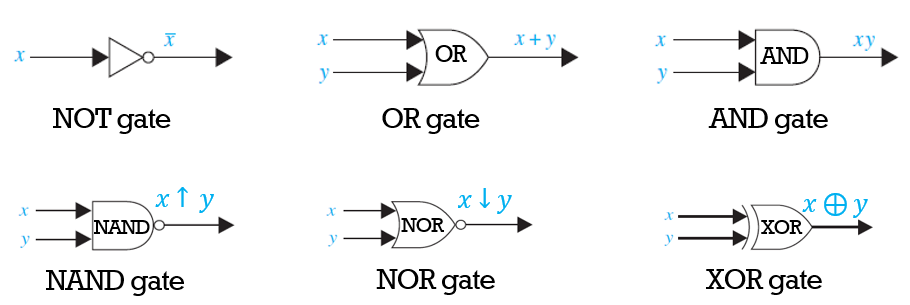
\includegraphics[width = 0.8\textwidth]{figure/gates.png} % Adjust width here to scale the image
    \caption{ANSI Symbols of Most Common Logic Gates. (\cite{rosen2012}).}
    \label{fig:gates}
\end{figure}

\textbf{\texttt{NOR} Logic Gates}\\
A \texttt{NOR} gate combines the characteristics of an \texttt{OR} gate with an inverter. The output of a \texttt{NOR} gate is 1 only when all inputs are 0. Any other input combination results in a 0 output.

\textbf{\texttt{XOR} Logic Gates}\\
An \texttt{XOR} (Exclusive OR) gate outputs a 1 only when exactly one of its inputs is 1. If both inputs are the same, either both 0 or both 1, the output will be 0. It functions like an \texttt{OR} gate, but with the additional condition that both inputs cannot be 1 simultaneously to produce a 1.

\textbf{\texttt{NAND} Logic Gates}\\
A \texttt{NAND} gate is a combination of an \texttt{AND} gate and a \texttt{NOT} gate. The output will be 0 only if all inputs are 1. In any other situation, the output will be 1.

Similarly to how we previously reduced Boolean expressions to simpler forms, we can achieve the same outputs using different circuit designs as seen in figure \ref{fig:gates2}.

\begin{figure}[h!]
    \centering
    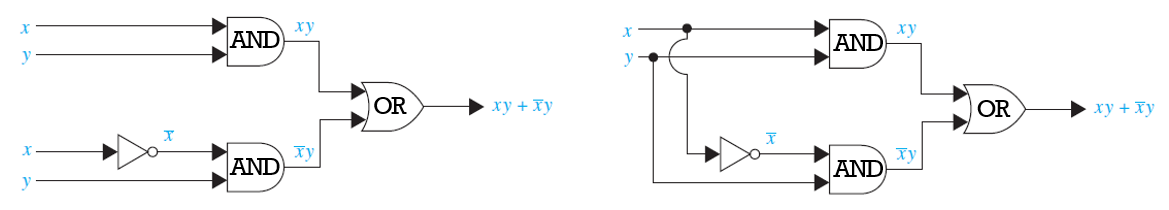
\includegraphics[width = 0.9\textwidth]{figure/gatessimilar.png} % Adjust width here to scale the image
    \caption{Two Equivalent Logic Gates. (\cite{rosen2012}).}
    \label{fig:gates2}
\end{figure}

We conclude this chapter by exploring the idea of \textbf{functional completeness}, also known as a \textbf{universal gate}. This concept refers to a set of logic gates that can be combined to implement any Boolean function. In essence, a functionally complete set of gates, like \texttt{NAND} or \texttt{NOR}, can replicate the behaviour of all other basic logic gates, making them versatile tools in digital circuit design.


\subsubsection*{Functional Completeness and a Universal Gate}
An operator or set of operators is considered \textbf{functionally complete} if it can be used to express any Boolean function. Both \texttt{NAND} and \texttt{NOR} gates are functionally complete, or \textbf{universal gates}, meaning that any logical expression can be constructed using only \texttt{NAND} or only \texttt{NOR}.

The reason the \texttt{NAND} (or the \texttt{NOR}) gate is functionally complete lies in its ability to mimic other Boolean operations. Using just \texttt{NAND} operations, we can construct the fundamental operations of \texttt{NOT}, \texttt{AND}, and \texttt{OR}, which are the building blocks for any Boolean function.

\begin{itemize}
\setlength{\itemsep}{10pt}
    \item \texttt{NOT} (\(\overline{x}\)): A \texttt{NOT} gate can be constructed by connecting both inputs of a \texttt{NAND} gate to the same variable:
    \(
    \overline{x} = x \uparrow x
    \)

    \item \texttt{AND} (\(x \cdot y\)): The \texttt{AND} operation can be achieved by first applying a \texttt{NAND} gate and then passing the result through a \texttt{NOT} (which, as seen, can also be constructed using \texttt{NAND}): \newline
   $x \cdot y=\overline{x \uparrow y}=(x \uparrow y) \uparrow(x \uparrow y)$

    \item \texttt{OR} (\(x + y\)): The \texttt{OR} operation can be created using multiple \texttt{NAND} gates, taking advantage of De Morgan’s laws:
    \(
    x + y = (x \uparrow x) \uparrow (y \uparrow y)
    \)
\end{itemize}


The table below demonstrates how we can construct the basic Boolean operations using only \texttt{NAND} gates. Notice how the different columns represent the transformations of variables $x$ and $y$ using combinations of \texttt{NAND} gates to form the logical operations \texttt{NOT}, \texttt{AND}, and \texttt{OR}:

\begin{table}[h!]
    \begin{center}
    \renewcommand{\arraystretch}{1.5} % Adjust this value for desired spacing
    \begin{tabular}{|c|c|c|c|c|}
    \textbf{Input} & \textbf{Input} & \textbf{NOT} & \textbf{AND} & \textbf{OR} \\
    $x$ & $y$ & $x \uparrow x$ & $(x \uparrow y) \uparrow (x \uparrow y)$ & $(x \uparrow x) \uparrow (y \uparrow y)$ \\
    \hline
    0 & 0 & 1 & 0 & 0 \\
    0 & 1 & 1 & 0 & 1 \\
    1 & 0 & 0 & 0 & 1 \\
    1 & 1 & 0 & 1 & 1 \\
    \end{tabular}
    \end{center}
    \caption{Constructing Basic Boolean Operators with \texttt{NAND} Gates.}
\end{table}

Since we have seen how to build all Boolean functions using just \texttt{NAND} gates, we now understand that all logic operations in a computer can be implemented using this single type of gate. This makes the \texttt{NAND} gate incredibly important in digital circuit design, as it allows for simpler and more efficient hardware implementation. In modern computer systems, transistors are used to build \texttt{NAND} gates, meaning that any logical operation can ultimately be represented by a combination of transistors.

\begin{figure}[h!]
    \centering
    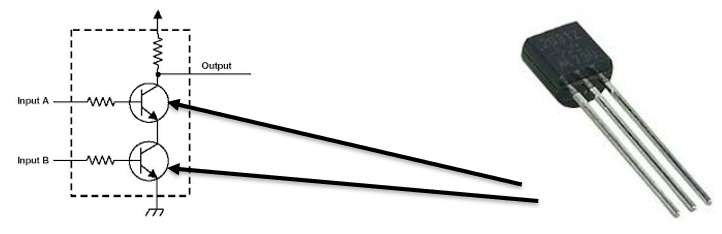
\includegraphics[width = 0.9\textwidth]{figure/logicincomp.png} % Adjust width here to scale the image
    \caption{Logic Gates in Computers.}
    \label{fig:logincom}
\end{figure}

Thus, the concept of functional completeness is not just theoretical; it is a powerful principle that allows computer engineers to design flexible and efficient circuits using minimal components.
